\chapter{The Optimality}

\vspace{1em}
\hfill
\begin{minipage}[c]{0.55\textwidth}
\raggedleft
\small\itshape
Solomonoff's distribution dominates any other computable distribution up to a multiplicative constant.\\[0.5em]
\upshape\footnotesize Marcus Hutter, \textit{Universal Artificial Intelligence} (2005)
\end{minipage}%
\hspace{0.5em}
\begin{minipage}[c]{0.12\textwidth}
% \includegraphics[width=\textwidth]{figures/ch05_optimality.png}
\end{minipage}
\vspace{1.5em}

\noindent Chapter 4 gave you a prior. It came from a counting argument on prefix-free codes: each program weighted by $2^{-|p|}$, summed over all programs producing the output $x$. The universal prior $M(x)$.

You can use $M$. You can also use something else.

The reason to use $M$ is a theorem.

\section*{The dominance theorem}

Let $\mu$ be any computable probability distribution on output strings. Any distribution that an algorithm can sample from, or compute the probability of. Most distributions of practical interest are computable. Gaussian, exponential, geometric. Every distribution a statistician has written down. Every distribution a physics calculation can produce.

The dominance theorem says: there is a constant $c_\mu$ such that

$$M(x) \geq c_\mu \cdot \mu(x)$$

for every string $x$.

In words: $M$ does not put substantially less probability on any string than $\mu$ does. Up to a multiplicative constant, $M$ contains $\mu$.

The constant is small. The constant does not depend on $x$. It depends only on $\mu$.

\section*{Why this is true}

The proof is a few lines.

Since $\mu$ is computable, there is a program that takes some randomness as input and outputs samples from $\mu$. The shortest such program has some length, the Kolmogorov complexity of $\mu$, written $K(\mu)$.

That program, in the universal Turing machine $U$, contributes weight $2^{-K(\mu)}$ to $M$. The contribution exists because $M$ is the sum over all programs producing each output, and the program that samples $\mu$ produces every output that $\mu$ assigns positive probability to, with the same relative frequencies.

So for each output $x$, the contribution from the $\mu$-sampling program to $M(x)$ is at least $2^{-K(\mu)} \cdot \mu(x)$. Other programs may also contribute, only adding to the total. Therefore

$$M(x) \geq 2^{-K(\mu)} \cdot \mu(x).$$

Figure~\ref{fig:dominance-proof} shows the inequality: the $\mu$-sampler's contribution alone, beside the full $M(x)$.

\begin{figure}[h]
\centering
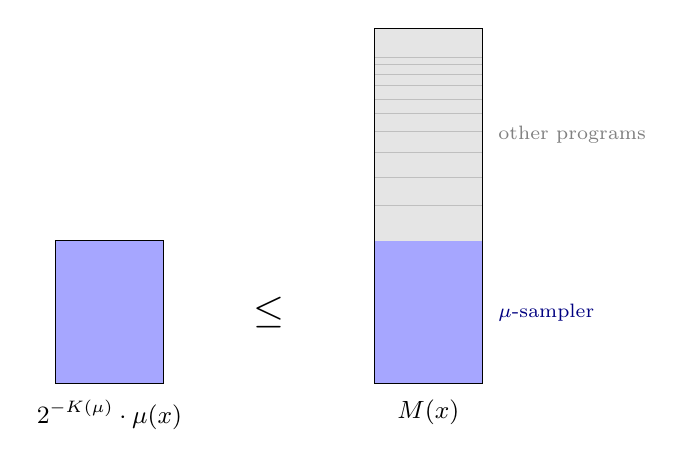
\begin{tikzpicture}[scale=0.9]
  % Bar 1: the μ-sampler's contribution alone
  \draw[thick] (0, 0) rectangle (1.5, 2);
  \fill[blue!35] (0, 0) rectangle (1.5, 2);

  % "≤" between bars
  \node[font=\Large] at (3, 1) {$\leq$};

  % Bar 2: M(x), with μ-sampler portion highlighted at bottom
  \draw[thick] (4.5, 0) rectangle (6, 5);
  \fill[blue!35] (4.5, 0) rectangle (6, 2);
  \fill[gray!20] (4.5, 2) rectangle (6, 5);
  % Internal dividers suggesting many other programs
  \draw[gray!50, thin] (4.5, 2.5) -- (6, 2.5);
  \draw[gray!50, thin] (4.5, 2.9) -- (6, 2.9);
  \draw[gray!50, thin] (4.5, 3.25) -- (6, 3.25);
  \draw[gray!50, thin] (4.5, 3.55) -- (6, 3.55);
  \draw[gray!50, thin] (4.5, 3.8) -- (6, 3.8);
  \draw[gray!50, thin] (4.5, 4.0) -- (6, 4.0);
  \draw[gray!50, thin] (4.5, 4.2) -- (6, 4.2);
  \draw[gray!50, thin] (4.5, 4.35) -- (6, 4.35);
  \draw[gray!50, thin] (4.5, 4.5) -- (6, 4.5);
  \draw[gray!50, thin] (4.5, 4.6) -- (6, 4.6);

  % Labels under bars
  \node[anchor=north, font=\small] at (0.75, -0.1) {$2^{-K(\mu)} \cdot \mu(x)$};
  \node[anchor=north, font=\small] at (5.25, -0.1) {$M(x)$};

  % Labels to the right of bar 2
  \node[anchor=west, font=\scriptsize, gray] at (6.1, 3.5) {other programs};
  \node[anchor=west, font=\scriptsize, blue!50!black] at (6.1, 1) {$\mu$-sampler};
\end{tikzpicture}
\caption{Why $M$ dominates $\mu$. The bar on the left is the contribution to $M(x)$ from the shortest program that samples $\mu$: weight $2^{-K(\mu)}$ times the frequency that program outputs $x$, which is $\mu(x)$. The bar on the right is the full universal prior $M(x)$: the sum of contributions from every program that produces $x$. The $\mu$-sampler is one of those programs. Many others contribute too. So $M(x)$ is at least as large as the $\mu$-sampler's piece alone.}
\label{fig:dominance-proof}
\end{figure}

The constant $c_\mu \approx 2^{-K(\mu)}$. Distributions that are short to describe (low $K(\mu)$) have a larger constant; $M$ is closer to them. Distributions that are long to describe have a smaller constant; $M$ is further from them. But every computable distribution is contained in $M$, with some constant.

\section*{What this means for prediction}

Solomonoff prediction is the procedure of conditioning $M$ on observations (Figure~\ref{fig:sequential-prediction}). The observed prefix is fed to $M$; the procedure returns a distribution over the next symbol. As the prefix grows, the distribution converges to the true conditional for any computable data source.

\begin{figure}[h]
\centering
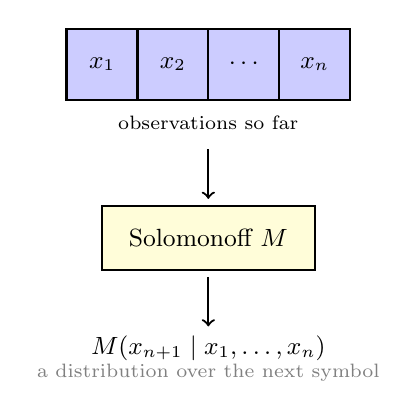
\begin{tikzpicture}[scale=0.9]
  % Input: observed prefix
  \foreach \i/\lbl in {0/{$x_1$}, 1/{$x_2$}, 2/{$\cdots$}, 3/{$x_n$}} {
    \draw[thick, fill=blue!20] (\i, 0) rectangle ({\i+1}, 1);
    \node[font=\small] at ({\i+0.5}, 0.5) {\lbl};
  }
  \node[anchor=north, font=\scriptsize] at (2, -0.1) {observations so far};

  % Arrow down to procedure
  \draw[->, thick] (2, -0.7) -- (2, -1.4);

  % Procedure box
  \draw[thick, fill=yellow!15] (0.5, -2.4) rectangle (3.5, -1.5);
  \node[font=\small] at (2, -1.95) {Solomonoff $M$};

  % Arrow down to output
  \draw[->, thick] (2, -2.5) -- (2, -3.2);

  % Output
  \node[anchor=north, font=\small] at (2, -3.2) {$M(x_{n+1} \mid x_1, \ldots, x_n)$};
  \node[anchor=north, font=\scriptsize, gray] at (2, -3.6) {a distribution over the next symbol};
\end{tikzpicture}
\caption{Sequential prediction. The observed prefix is fed to the procedure; the procedure returns a distribution over the next symbol. As the prefix grows, the distribution converges to the conditional under the true generative process.}
\label{fig:sequential-prediction}
\end{figure}

The bound on the total error comes directly from the dominance theorem. Take logarithms of $M(x) \geq 2^{-K(\mu)} \cdot \mu(x)$:

$$\log_2 \mu(x) - \log_2 M(x) \leq K(\mu).$$

By the chain rule for log-probabilities, the left side equals the cumulative gap between $\mu$ and $M$ summed over every step of the sequence. So the total excess log-loss of using $M$ in place of $\mu$, over a sequence of any length, is bounded by $K(\mu)$ bits.

The bound does not depend on the length of the sequence. No matter how many observations you make, the total cost of using $M$ instead of $\mu$ never exceeds $K(\mu)$. The per-observation cost, then, goes to zero as the sequence grows. Solomonoff catches up. Figure~\ref{fig:dominance} shows the convergence.

\begin{figure}[h]
\centering
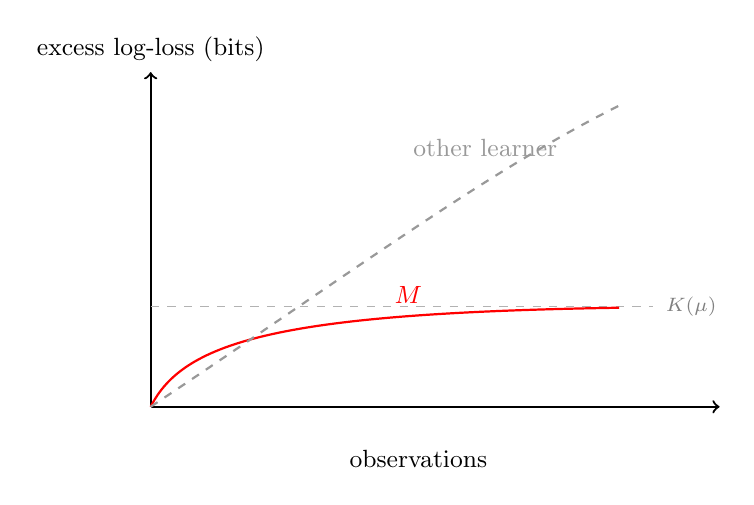
\begin{tikzpicture}[scale=0.85]
  % Axes
  \draw[->, thick] (0, 0) -- (8.5, 0);
  \draw[->, thick] (0, 0) -- (0, 5) node[above, font=\small] {excess log-loss (bits)};

  % Asymptote line
  \draw[dashed, gray!60] (0, 1.5) -- (7.5, 1.5);
  \node[anchor=west, font=\scriptsize, gray] at (7.55, 1.5) {$K(\mu)$};

  % M's curve: asymptotes to the constant
  \draw[thick, red] (0, 0) .. controls (0.5, 1) and (2, 1.4) .. (7, 1.48);
  \node[anchor=south west, font=\small, red] at (3.5, 1.4) {$M$};

  % Other learner: grows
  \draw[thick, dashed, gray!80] (0, 0) .. controls (3, 2) and (5, 3.5) .. (7, 4.5);
  \node[anchor=south, font=\small, gray!80] at (5, 3.6) {other learner};

  % X-axis label
  \node[anchor=north, font=\small] at (4, -0.5) {observations};
\end{tikzpicture}
\caption{Why $M$ is optimal. The curves show excess cumulative log-loss compared to the true distribution $\mu$, measured in bits, as a function of observations. Solomonoff's prediction $M$ asymptotes to the constant $K(\mu)$: its total mistake against the true distribution is bounded by the description length of $\mu$. Other computable learners can have excess loss that grows without bound. As data accumulates, the per-observation penalty for using $M$ goes to zero.}
\label{fig:dominance}
\end{figure}

This is the optimality. Solomonoff catches up to any computable distribution, with a penalty that does not grow with data. ``Shorter is more probable'' is the reason. The dominance theorem makes the simplicity bias an optimality property, not an aesthetic one.

\section*{The choice of machine}

The construction of $M$ depended on a choice of universal Turing machine $U$. A different machine $U'$ gives a different prior $M'$.

The invariance theorem says it does not matter.

For any two universal Turing machines $U$ and $U'$, there exists a constant $c$ such that

$$M(x) \leq c \cdot M'(x) \quad \text{and} \quad M'(x) \leq c \cdot M(x)$$

for all $x$. The constant is determined by the length of the shortest cross-compiler from $U$ to $U'$ (and back). For any reasonable pair of universal machines, this is a few hundred bits at most.

So: in the limit of large data, the choice of $U$ produces a constant-factor difference and nothing more. The universal prior is well-defined up to a constant. The constant does not depend on $x$, does not grow with data, and becomes negligible compared to the bits of information that data carries.

This matters more philosophically than practically. Philosophically: ``the universal prior'' is not a thousand priors competing on equal terms. It is one object, with a well-defined notion of equivalence across machines. Practically: in any specific calculation, you pick a $U$ and stay with it.

\section*{The bedrock, complete}

The bedrock of inference under uncertainty is now in place. Four ingredients:

\begin{itemize}
\item \textbf{Cox's theorem.} The unique calculus of belief is probability theory.
\item \textbf{Bayes' theorem.} The unique update rule is conditional probability, derived from counting in a restricted subset.
\item \textbf{Kraft's inequality plus the universal prior.} The unique prior, up to a constant, is the one that weights computable programs by $2^{-|p|}$.
\item \textbf{Dominance and invariance.} The universal prior catches up to any computable prior, and the choice of machine is asymptotically irrelevant.
\end{itemize}

Each piece is settled mathematics. None of it is in dispute. Together, the four pieces specify what optimal learning under uncertainty looks like. An agent that does substantially better than this on computable data does not exist.

\section*{The bedrock in the wild}

This is mathematics from the 1960s. Sixty years ago, it was an abstract result, of interest mainly to a handful of researchers in computability and information theory.

It is no longer abstract.

Modern language models are bounded computable approximations of the universal prior over text. They are trained on trillions of words and are asked, during training, to predict the next token given the previous ones. This is the same thing as minimizing description length: the number of bits required to encode the data given the model. The loss measures, exactly, how far the model's distribution is from optimal. Models with lower loss are closer to the universal distribution over the text they were trained on.

The dominance theorem predicts the behavior. A larger model, with more parameters, can represent a richer set of computable distributions, and so its training loss approaches the loss of the (unknown) generative process more closely. Scaling laws are the empirical confirmation. As the model grows, the gap to optimal shrinks at a measurable rate, and the rate is the kind of constant-bounded convergence the dominance theorem promises.

Acting, not just predicting, is also covered. In 2005, Marcus Hutter defined AIXI: the optimal agent that uses the universal prior for belief and selects actions to maximize expected discounted reward. AIXI is uncomputable, like $M$, but bounded approximations exist. A language model that has been fine-tuned with reinforcement learning is a practical implementation of the AIXI picture. The base model is the Solomonoff predictor. The reinforcement signal pushes the model toward an objective. The combination is a finite-resource approximation of the optimal learner-and-actor.

The failures of these systems, when they fail, are Russell's-chicken failures. They extrapolate confidently from a pattern in their training data; the world is more complicated than the pattern suggested; the extrapolation is wrong about the moment that matters. They are not failing because the mathematics is wrong. They are failing because they are bounded approximations, and the world contains structure the approximation does not see. The chicken's reasoning was sound given its data. Modern models reason soundly given theirs. The bound is what costs.

This is the bedrock confirmed at civilizational scale. Mathematics from 1964, applied to a trillion words and a million GPUs, produces the behavior the mathematics predicts.

\section*{Where this leaves you}

The mathematics of optimal learning is closed. Bayes' theorem, the universal prior, the dominance theorem, the invariance theorem. Each piece is a theorem. Each derivation is short. The package is settled.

What remains is interpretation.

So far, the universal prior has been a distribution on hypotheses. A way of weighting candidate explanations of the data you have. The next chapter takes a step the mathematics does not force, and watches what happens to the picture when it is taken.
